%%%%%%%%%%%%%%%%%%%%%%%%%%%%%%%%%%%%%%%%%
% Thin Sectioned Essay
% LaTeX Template
% Version 1.0 (3/8/13)
%
% This template has been downloaded from:
% http://www.LaTeXTemplates.com
%
% Original Author:
% Nicolas Diaz (nsdiaz@uc.cl) with extensive modifications by:
% Vel (vel@latextemplates.com)
%
% License:
% CC BY-NC-SA 3.0 (http://creativecommons.org/licenses/by-nc-sa/3.0/)
%
%%%%%%%%%%%%%%%%%%%%%%%%%%%%%%%%%%%%%%%%%

%----------------------------------------------------------------------------------------
%	PACKAGES AND OTHER DOCUMENT CONFIGURATIONS
%----------------------------------------------------------------------------------------

\documentclass[article, 11pt]{article} % Font size (can be 10pt, 11pt or 12pt) and paper size (remove a4paper for US letter paper)

\usepackage[protrusion=true,expansion=true]{microtype} % Better typography
\usepackage{graphicx} % Required for including pictures
\usepackage{wrapfig} % Allows in-line images
\usepackage[margin=1.25in]{geometry}
%\graphicspath{ {/Users/jms3917/Desktop/NYCEM/report/images/} }

\usepackage[scaled]{helvet} % Use the Helvetica font
\renewcommand\familydefault{\sfdefault} 
\usepackage[T1]{fontenc} % Required for accented characters

\usepackage{mathpazo} 
\usepackage[T1]{fontenc} 
\linespread{1.05} % Change line spacing here, Palatino benefits from a slight increase by default

\makeatletter
\renewcommand\@biblabel[1]{\textbf{#1.}} % Change the square brackets for each bibliography item from '[1]' to '1.'
\renewcommand{\@listI}{\itemsep=0pt} % Reduce the space between items in the itemize and enumerate environments and the bibliography

\renewcommand{\maketitle}{ % Customize the title - do not edit title and author name here, see the TITLE block below
\begin{flushright} % Right align
{\LARGE\@title} % Increase the font size of the title

\vspace{50pt} % Some vertical space between the title and author name

{\large\@author} % Author name
\\\@date % Date

\vspace{40pt} % Some vertical space between the author block and abstract
\end{flushright}
}

%----------------------------------------------------------------------------------------
%	TITLE
%----------------------------------------------------------------------------------------

\title{\textbf{New York City Economic Map}\\ % Title
Applied Urban Science \& Informatics Capstone} % Subtitle

\author{\textsc{Tong Jian, Kenneth Luna, Samuel Pollack \& Julia M. Smith} % Author
\\{\textit{M.S. Candidates, NYU Center for Urban Science + Progress}}} % Institution

\date{\today} % Date

%----------------------------------------------------------------------------------------

\begin{document}

\maketitle % Print the title section

%----------------------------------------------------------------------------------------
%	ABSTRACT AND KEYWORDS
%----------------------------------------------------------------------------------------

%\renewcommand{\abstractname}{Summary} % Uncomment to change the name of the abstract to something else

\begin{abstract}
The New York City Economic Map (NYCEM) is an interactive tool that provides insight to economic activity across New York City census tracts by both querying relevant statistics and clustering key employment features. The understanding of variations in demographics, industry patterns, and employment trends across New York City census tracts is critical to the development of effective civic programs. Thus, NYCEM's intention is to provide a method for visualizing and comparing business-related activity in order to most effectively target small business outreach and support services. On behalf of New York City Small Business Services and Citi's Community Development branch, NYCEM provides a proof-of-concept study in support of ongoing small business development initiatives. 
\end{abstract}

\hspace*{3,6mm}\textit{Keywords:} New York City, economic, map, small business% Keywords

\vspace{30pt} % Some vertical space between the abstract and first section

%----------------------------------------------------------------------------------------
%	ESSAY BODY
%----------------------------------------------------------------------------------------

\section*{Objective}

The New York City Economic Map (NYCEM) has been undertaken as a capstone project following last year's development of a New York City Economic Profile. At present, the project is an internal research initiative advised by Dr. Greg Dobler and Dr. Tim Savage. In early May 2015, NYCEM advisors met with representatives from Citi's Community Development branch (Citi) and New York City Small Business Services (SBS). These two stakeholders have launched a historic partnership which seeks to identify and target minority-owned businesses to best extend existing and newly developed small business support services. The purpose of the meeting was to gauge the partnership's interest in NYCEM and understand which research direction would best cater to their objectives The partnership expressed interest in identifying and profiling businesses in predominantly minority and low-income neighborhoods. These findings will ideally inform their outreach strategy and enhance take-up of existing and newly developed services. 
\\\\
Research into existing services showed that small business outreach events and trainings were predominantly held in community centers and open to all existing or potential small business owners. While certainly inclusionary, take-up of services may be enhanced through a more targeted strategy that pinpoints exact census tracts. For instance, in census tracts with a recent spike in the number of pizza establishments, targeted services might include business plan development with an emphasis on differentiation in order to distinguish each business from the competition and capture requisite market demand.
\\\\
Below is the low-to-moderate income (LMI) criteria that Citi is bound to in their consideration of small business development initiatives:
\begin{enumerate}
\item "An individual is considered 'low-to-moderate income' (LMI) if his or her household Income is \$55,113 or below, which is less than 80 percent of the New York-Jersey City-White Plains, NY-NJ Metropolitan Statistical Areas (MSA code 35614) Federal
Financial Institutions Examination Council (FFIEC) estimated 2014 Median Family Income of \$68,900."
\item "A small business meets the 'economic development' criteria if it earns \$1 million or less in annual gross revenue and one of the following two criteria is also true:
The business supports permanent job creation/retention/improvement for low-to-moderate (LMI) income individuals and/or the business is located in a low-to-moderate (LMI) income census tract, or is a government-targeted redevelopment area."
\end{enumerate}
In responding to Citi's request for proof-of-concept studies, the team's strategy evolved into the development of a queryable database of small business activity in New York City where information is translated visually onto an interactive map. The database includes demographic, industry, and employment figures across New York City census tracts. Upon selecting an industry, NYCEM provides summary statistics for the census tract, including median household income and median business revenue. At present, the NYC Business Atlas provides similar summary statistics at a granular level to cater to potential small business owners during the development of a business plan. NYCEM expands on this functionality by providing employment comparisons across industries. Each census tract is assigned a cluster number, 1-5, and when selected shows a plot of employment by industry across similar census tracts. Perhaps most interesting to stakeholders such as SBS and Citi is NYCEM's depiction of activity within the census tract over time. The database includes five years of demographic data, so recognized changes in industry or employment distributions can be easily compared to related demographic trends.
\\\\
This document details NYCEM's trajectory from April 2015 to July 2015. The project was submitted to advisors Dr. Greg Dobler and Dr. Tim Savage of the New York University Center for Urban Science + Progress on July 29, 2015.

%------------------------------------------------
\section*{Context}

Beyond conveying the results of demographic and industry queries at the census tract level, the team has sought to understand what measures have come to quantify business success. This conversation was primarily informed by related academic texts.
\\\\
In 1990, economists Steven J. Davis and John Haltwanger from the University of Chicago Graduate School of Business and the University of Maryland summarized baseline workforce trends, such as the propensity for job separation following a year of work and routine turnover within an establishment. The team noted that these trends have vast macroeconomic impact when experienced across all firms. The authors found that costs associated with churn, hiring, and displacement all posed significant friction for individual firms. \cite{Davis} This friction can largely be credited for more robust market dynamics in periods of flux. These findings have become increasingly relevant to today's start-up laden market, where individual business interests catalyze widespread hiring sprees but often result in buy-outs or closures in the wake of fierce industry competition.
\\\\
In a further attempt to understand the impact of firm size on the economy, John Haltiwanger collaborated with Ron S. Jarmin and Javier Miranda in 2013 to investigate a commonly held belief which largely impacts public policy: that small businesses employ the most employees. Using the Census' Longitudinal Business Database, there was a subtle inverse relationship between firm size and net growth, which supports this belief. However, once controlling for firm age, this relationship disappeared and in some cases reversed (which can be attributed to high separation at small firms.) The authors found that firms over 10 years old with greater than 500 employees account for about 45 percent of all jobs in the U.S. private sector. These mature firms comprise nearly 40 percent of job creation and destruction and resulting job creation and destruction across employer size cohorts approximated their proportion of total employment. An exception, however, is that start-ups comprise only 3 percent of total employment but represent nearly 20 percent of gross job creation. \cite{Haltiwanger} These findings seem to herald the importance of start-ups and the catalytic potential in fostering their success.
\\\\
To understand this diversity of findings, a follow-up publication by John Haltiwanger, Ryan Decker, Ron Jarmin, and Javier Miranda from 2014 attempts to quantify the impact of start-ups' employment, and finds the resulting analysis to be inconclusive. Their most recent findings illustrate that many start-ups do not succeed, yet the few that do contribute disproportionately in terms of employment and revenue. These baseline findings complicate policy recommendations which seek to prioritize the growth of potentially high-impact new companies. The primary take away is that start-ups initially hire disproportionately, and thus their failures are more pronounced given frequent firm turnover amongst this cohort. \cite{Decker} 
\\\\
As a result of these findings, our team identified business tenure as the primary indicatory of long-term business success, and resultantly more stable employment. Unfortunately, publicly available data at the requisite level of granularity does not currently hold a measure of business tenure.

%------------------------------------------------

\section*{Data Sources}

Data has been pulled from four primary sources, three publicly available and one commercially available. Demographic data originates from the most recent American Community Survey from years 2009 to 2013 which includes relevant information such as household income, race, and geography to the census tract level. Employment by industry data from 2012 was obtained from the Census Longitudinal Employer-Household Dynamics (LEHD) Original-Destination Employment Statistics (LODES). Relying heavily on public data, this project supports New York City's open data and analytics initiatives. 
\\\\
Private data for this project has been procured by NYU from ReferenceUSA, a data provider which has collected and tabulated survey responses of business profiles with employee count and associated revenue to a very granular level across the years 2010 to 2014. The exact name and address of each surveyed business is included in the data set leading to increased privacy concerns and necessitating the need for dedicated local machines for storage and analysis during the course of the project. ReferenceUSA data was aggregated and compared to Census' Zip Code Business Patterns in order to gauge the degree to which the survey deviated from the known universe of businesses defined by the Census. 

%------------------------------------------------

\section*{Data Exploration}

Initial efforts concentrated on understanding nuances between publicly available data sets and their role within the overarching project objectives. 
\\\\
Using Census Zip Code Business Patterns for 2012, the team aggregated establishment count into three bins based on a coordinated understanding of the business sizes that garner City interests: the smallest employee count bin with 0-49 employees, the mid-size employee count bin with 50-249 employees, and the largest employee count bin with 250+ employees. When normalizing business sizes by total establishments, a choropleth revealed that all zip codes in New York are comprised of at least 70\% small businesses. [Figure 1] Clusters of small business activity was predominantly seen in the Lower East Side and East Village zip codes, as well as the majority of Southern Brooklyn, where percentages of businesses with less than 50 employees climb to the high 90\% range of total establishments. 
\\\\
Next, using an unsupervised learning tool, k-means clustering, the zip codes were clustered according to feature similarities. The unique attribute is zip code and the features considered were the percentage of small, medium, and large businesses within each geography. [Figure 2] It is important to note that these centroids are not contained within the data set but are instead the mean of the features within the cluster. As such, the centroid of each cluster provides a profile that is the average of the cluster's business compositions. The centroids of business compositions for each of four clusters were located at the following points:
\begin{enumerate}
\item Small Businesses 94.30\%, Mid-Size Businesses: 4.85\%, Large Businesses: 0.85\%
\item Small Businesses 97.76\%, Mid-Size Businesses: 1.93\%, Large Businesses: 0.31\%
\item Small Businesses 81.33\%, Mid-Size Businesses: 13.81\%, Large Businesses: 4.85\%
\item Small Businesses 89.21\%, Mid-Size Businesses: 9.21\%, Large Businesses: 1.58\%
\end{enumerate}
The cluster centroids indicate that while each zip code contains at least 70\% small businesses, the mean of each centroid represents at least 81.33\% small businesses. Additionally, though spatial constraints were not enforced during processing, it is apparent that many clusters are geographically contiguous. This leads to the notion that business profiles are often similar in proximate zip codes, likely due to shared features such as a common customer base.
\\\\
For each of the three previously-defined business size categories - small, mid-size, and large - k-means clustering was next conducted on the absolute number of businesses with time over the last ten years, 2002 to 2013. Each zip code observed has been defined by ten years of features for each business type, or in the other words the count of that business type across ten years. [Figure 3] After parsing the data into three unique data frames for counts of small, mid, and large business counts these ten dimensional feature vectors have been normalized by subtracting the mean and dividing by the standard deviation of aggregate business counts within each year across all zip codes. [Figure 4]
\\\\
When considering the distribution of unique businesses in each NAICS sub-category, the team devised a histogram that shows a highly skewed distribution with several outliers. [Figure 5] These outliers can likely be attributed to the food and beverage sectors and key New York City industries, such as finance, which account for thousands of firms. 
\\\\
Moving beyond publicly available Census data, the team explored ReferenceUSA's Business Historical Data for the years 2010 through 2014. ReferenceUSA purports to be a small business survey that collects voluntary data from business owners related to employment, tenure, and revenue. Grouping by business type for one year, it was found that medical practices are the biggest cohort by far. This might be a concern as small law and medical practices are exactly that, practices instead of small businesses. Next, when considering sales volume by employees across industries, it was found that the highest performing business types were petrol stations and refineries, which led the team to believe that larger conglomerates that are oil-based were also included in the data set. To round out ReferenceUSA summary statistics and data exploration, histograms of sales volume were devised to demonstrate which revenue bins contained the highest number of unique businesses. At this point, the team filtered out all businesses that fell outside the 90th percentiles to avoid heavily skewed outputs. [Figure 6] Resultantly, the \$500,000 per year revenue range was found to contain the highest number of businesses.

%------------------------------------------------

\section*{Data Limitations}

The limitations of each data set are apparent: open data does not reach the level of granularity needed to produce a map at the block or lot level, and the private data, though robust in fields, is lacking in the number of businesses surveyed. Because many businesses do not have the time or inclination to respond, and those that do respond are self-reporting their revenue figures, there is a high chance that the responses are skewed in favor of high-revenue practices with administrative support. 
\\\\
In an effort to quantify variance between ReferenceUSA's survey and the Census' Zip Code Business Patterns, the team devised a plot to demonstrate where employee counts varied significantly between the two sources. [Figure 7] Poor responses were generally seen in less affluent neighborhoods such as Central Brooklyn, Eastern Queens, and Washington Heights. Unfortunately, many zip codes also reflected positive variations in percentages, which demonstrated that ReferenceUSA contained more survey responses per zip code than were included in the Census Zip Code Business Patterns subset of business counts with less than 50 employees. Inclusion of "large" small businesses coupled with low response rates and liberal figure estimates are the causes we hypothesized would lead to significant inaccuracies when relying on the ReferenceUSA data.

%------------------------------------------------

\section*{Analytical Methods}

Data wrangling efforts for construction of the central NYCEM database concentrated on aligning our available data sources in order to compile a single table that will inform future querying and geographic representation. The first filter required removing businesses in ReferenceUSA that were not located within the five boroughs. ReferenceUSA data contained several businesses with latitudes and longitudes that place them in eastern Long Island and parts of New Jersey. After removing non-NYC based businesses, data was joined at the census tract level to include the Standard Industrial Classification (SICD), Primary NAICS Title Lable (PNATITL), county/borough, and census tract and the sum and median of both annuals sales volume and employee count were extrapolated. The median was used instead of the average to address several businesses that do not fall within the definition of small businesses. For example, a business such as Bank of America with several hundred millions of dollars in annual revenue and thousands of employees far exceed the threshold of small businesses.
\\\\
The resulting dataframe provided a hierarchy of summary statistics at the census tract level. To clarify, the PNATITL code is a broader category than the SICD code. The dataset in this form contained 4,500+ SICD codes grouped into 940+ PNATITL codes. Unfortunately, we felt that this level of granularity would be too much for our use-case, therefore we appended one of the 24 NAICS codes to each PNATITL-SICD combination. This data structure allowed us to present users with higher-level categorizations, and iteratively work their way down to the appropriate business category.
\\\\
After merging the NAICS codes, we proceeded to append the shapefile polygons for the census tract linked to each NAICS-PNATIL-SICD combination. The first step was reading the NYC census tract shapefiles using GeoPandas. The dataframe loaded via GeoPandas contained the borough and census tract code for each polygon; these two attributes were used to append the polygon points. This dataframe contains over 150 thousand observations for each year between 2010 and 2014 and, with the inclusion of the polygon points, is too large to convert into a GeoJson file. To work around this issue, we decided to create a hierarchy of directories based on the NAISC, PNATITL, and SICD codes. This kept our Mapbox visualization from having to load and parse an extremely large file which can be too expensive for the front-end. For example, mobile food trucks would fall into the following hierarchical directory structure: ~/2010/ACCOMMODATION AND FOOD SERVICES/MOBILE FOOD SVCS. Another example would be vocational computer training courses: ~/2010/EDUCATIONAL SERVICES/COMPUTER TRAINING. Again, the hierarchy of data is first the year, NAICS, SICD, followed by the GeoJson file for SICD code.
\\\\
The GeoJson files contains polygon points for each census tract but also other attributes specific to that business category in that area. The following is a list of all attributes and their definitions which are provided in the queryable database:
\begin{itemize} 
\item SLSVDT\_SUM: Aggregate sales volume by business type in census tract (CT)
\item SLSVDT\_MED: Median sales volume by specific business type in CT
\item EMPSDT\_SUM: Aggregate number of employees by specific business type in
CT
\item EMPSDT\_MED: Median number of employees per business for specific business
type in CT
\item COUNT\_SUM: Number of businesses to fall in specific business type in CT
\item SHAPE\_AREA: Area of CT in square feet
\item GEO\_COUNTY: Borough/county code
\item SHP\_BOROUGH: Borough/county name
\item SHP\_CENSUS\_TRACT: CT number
\item NTANAME: Neighborhood name
\item NAICS\_LABEL: North American Industry Classification System code
\item PNACODE: Primary NAICS code
\item PNATITL: Primary NAICS Title label
\item PRMSIC: Standard Industrial Classification code
\item SICD: Standard Industrial Classification
\item LMI\_CT: Median Household Income from ACS-5 Year (07-11) ***
\item LMI: Column at \$55,113 to facilitate the parsing of census tracts to those below this benchmark, shown in red below.
\item LODES: Clusters 0-4 representing 5 unique clusters of employment counts across industries, later numbered 1-5
\end{itemize}
\pagebreak

%------------------------------------------------

\section*{Mapping Visualization}

Upon running the mapping visualization locally (available at http://github.com/gdobler/nycem), the user is able to select census tracts and view summary statistics from the database on the side panel. Perhaps most central to understanding the business context within each census tract is an understanding of how that census tract compares across New York City. Using ACS 2009-2013 estimates, the team noted in the summary panel whether Census tract median household income was located above or below the median household income threshold identified by Citi, \$55,113. [Figure 8] Next, when the user clicks on either the side panel or the census tract within view, a pop-up is generated that provides relevant employment statistics from LODES. [Figure 9] Beyond querying, this LODES information has been clustered using k-means in order to identify census tracts that have experienced similar employment patterns. [Figure 10]
\\\\
The map design and data layering is all created using Mapbox and the Leaflet API. [Figure 11] MapBox, an open source platform for customized mapping, provided template and the team and added custom design features such as drop down menus and call-outs. The database has been coded as GeoJsons which are read into the map using a function from Leaflet. Using Javascript/JQuery, sub-sections of the HTML page are selected in order to store user clicks into global variables. These global variables are then concatenated to form the URL and directory where the geojson files are stored. Additional map functionality is provided by HTML and CSS. The maps drop-down menus are powered by Twitter Bootstrap, which allows for custom design.

%------------------------------------------------

\section*{Future Work}

In accordance with existing literature on business success, the team sought data on business tenure but was unable to locate a publicly available source at the census tract level. Future work should prioritize research into this type of source in order to more effectively project business success. Additionally, consideration of registered MWBE businesses using the City's VENDEX database would allow for exploration of resulting revenues generated from publicly-contracted work. This type of research might lead to a better understanding of what factors incentivize MWBE businesses to contract with the City, and quantify the results of this collaboration.

\section*{Contributions}

Data exploration was undertaken jointly by Kenneth Luna and Julia M. Smith. Domain research was compiled by Julia M. Smith. Data wrangling and database development was led by Kenneth Luna with support from Samuel Pollack. Employment clustering was led by Tong Jian. Static mapping was completed by Julia M. Smith. Mapping visualization was undertaken jointly by Samuel Pollack and Kenneth Luna. Project management and deliverables preparation was led by Julia M. Smith. 

%------------------------------------------------
\pagebreak

\begin{thebibliography}{100}
\bibitem{Davis} Davis, S., Haltiwanger, J., `Gross Job Creation, Gross Job Destruction, and Employment Reallocation," \emph{University of Chicago and University of Maryland}, 1990.
\bibitem{Haltiwanger} Haltiwager, J., Jarmin, R., and Miranda, J., ``Who Creates Jobs? Small vs. Large vs. Young," \emph{The Review of Economics and Statistics}, 2013.
\bibitem{Decker} Decker, R., Haltiwanger, J., Jarmin, R., and Miranda, J. ``The Role of Entrepreneurship in U.S. Job Creation and Economic Dynamism," \emph{Journal of Economic Perspectives}, pp. 3-24, 2014.
\end{thebibliography}

%------------------------------------------------

\subsection*{Figure 1}
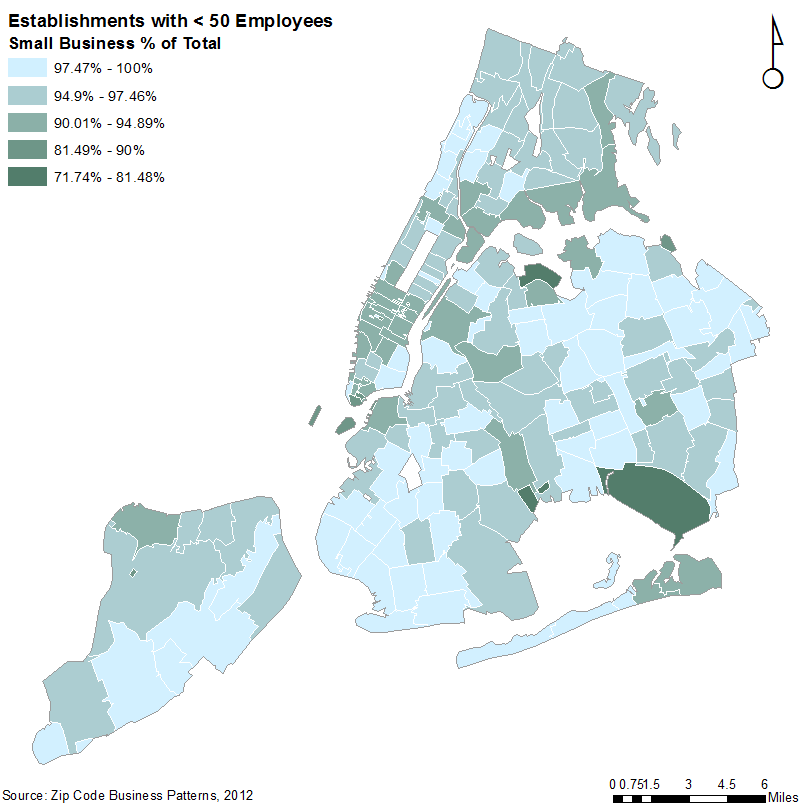
\includegraphics[width=1.0\textwidth]{1}
\\\\
\pagebreak
\subsection*{Figure 2}
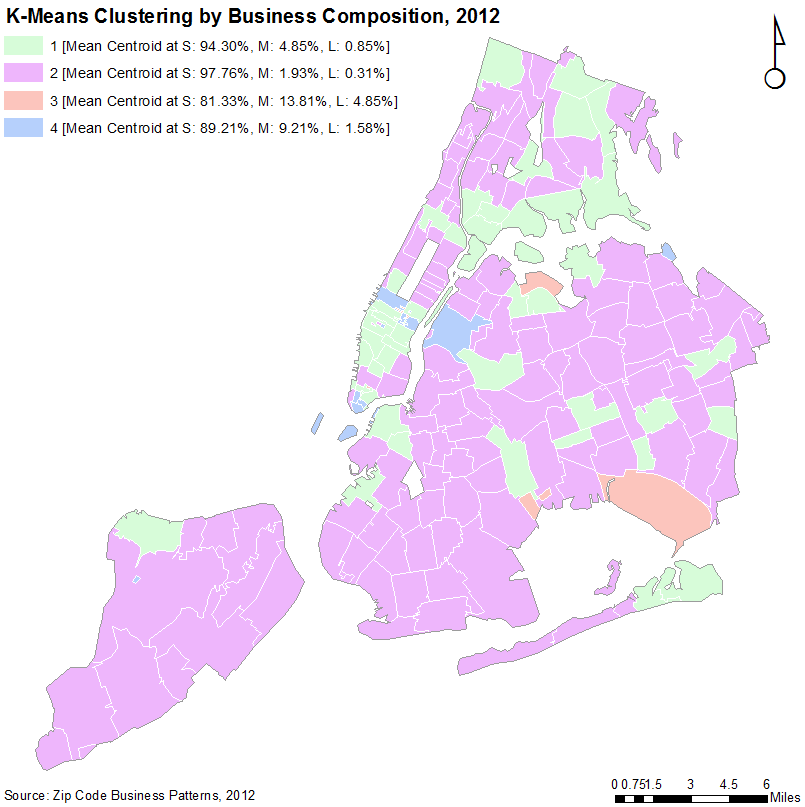
\includegraphics[width=1.0\textwidth]{2}
\pagebreak
\subsection*{Figure 3}
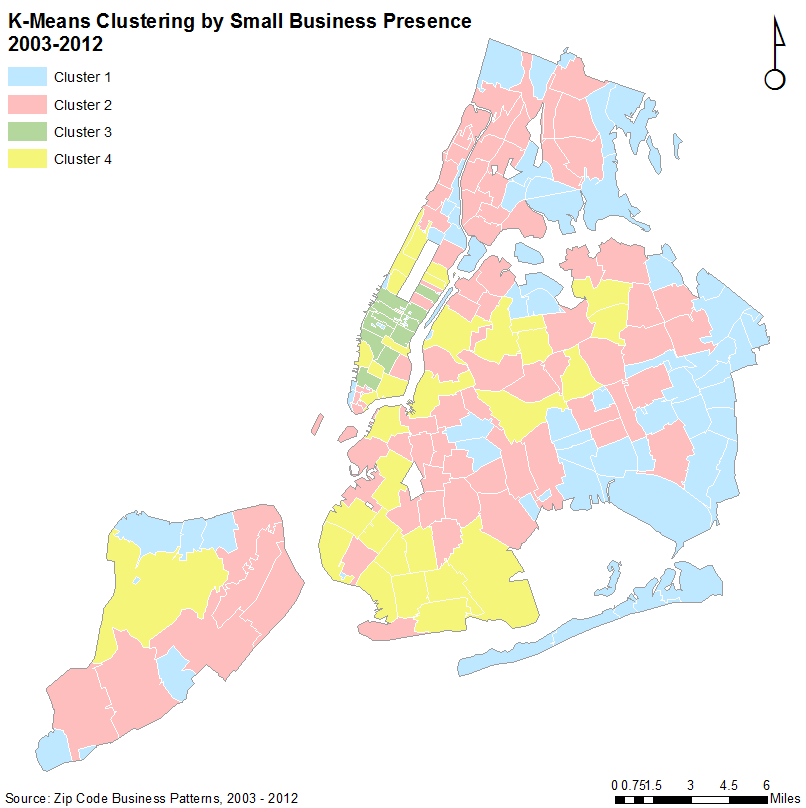
\includegraphics[width=1.0\textwidth]{3}
\pagebreak
\subsection*{Figure 4}
\hfill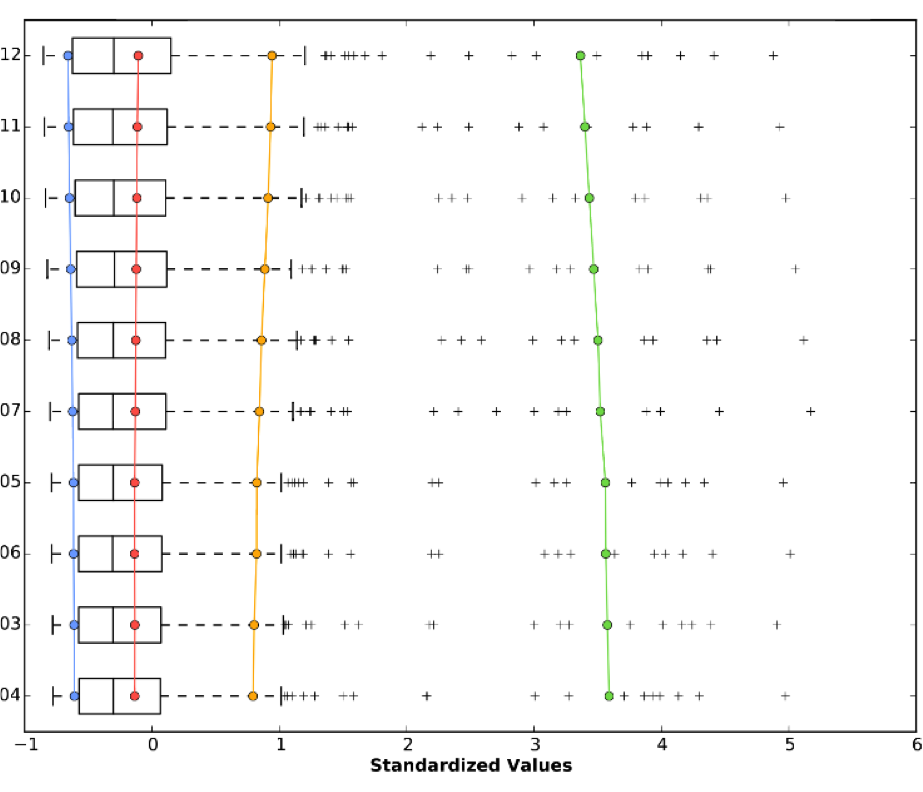
\includegraphics[width=.95\textwidth]{4}\hspace*{\fill}
\subsection*{Figure 5}
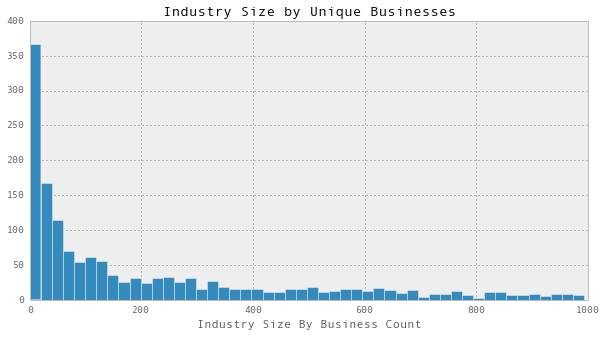
\includegraphics[width=1.0\textwidth]{5}
\pagebreak
\subsection*{Figure 6}
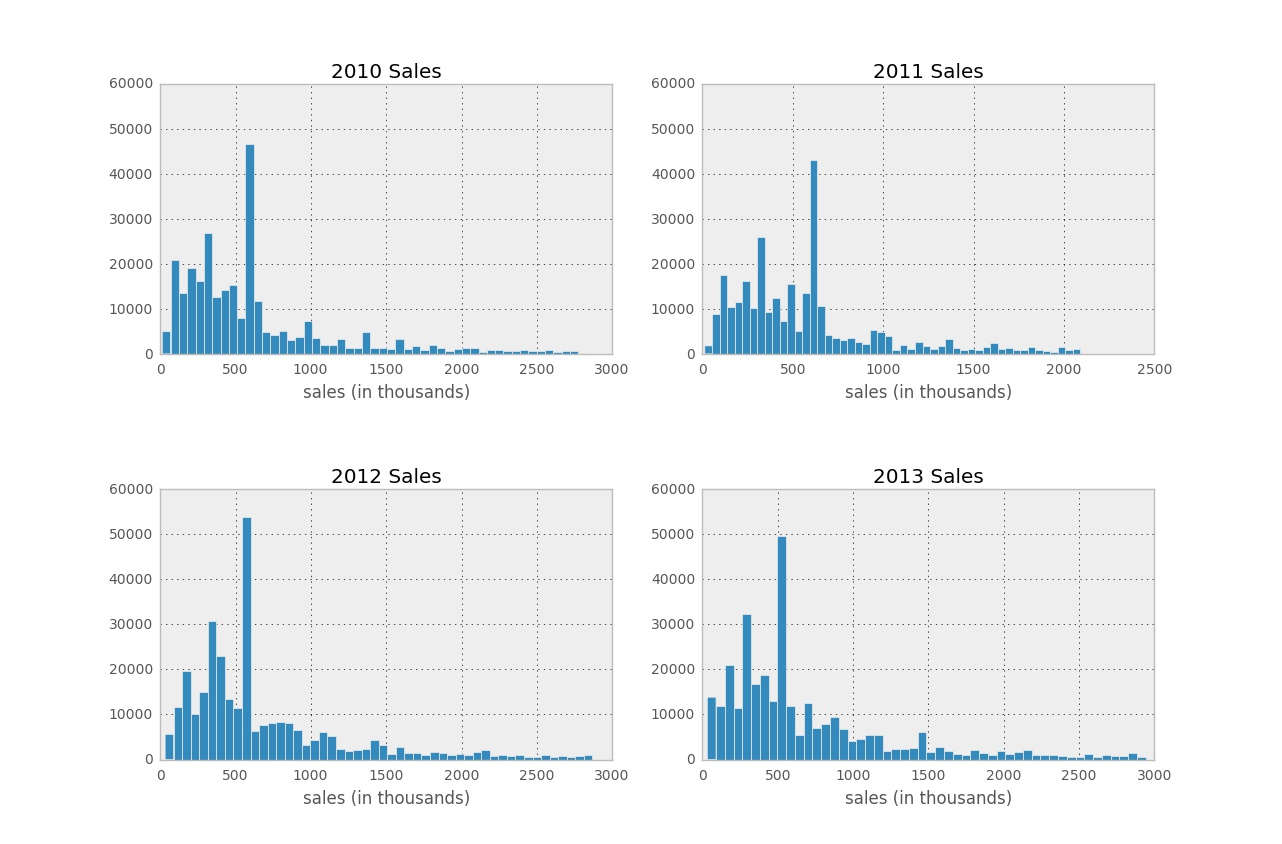
\includegraphics[width=1.0\textwidth]{6}
\pagebreak
\subsection*{Figure 7}
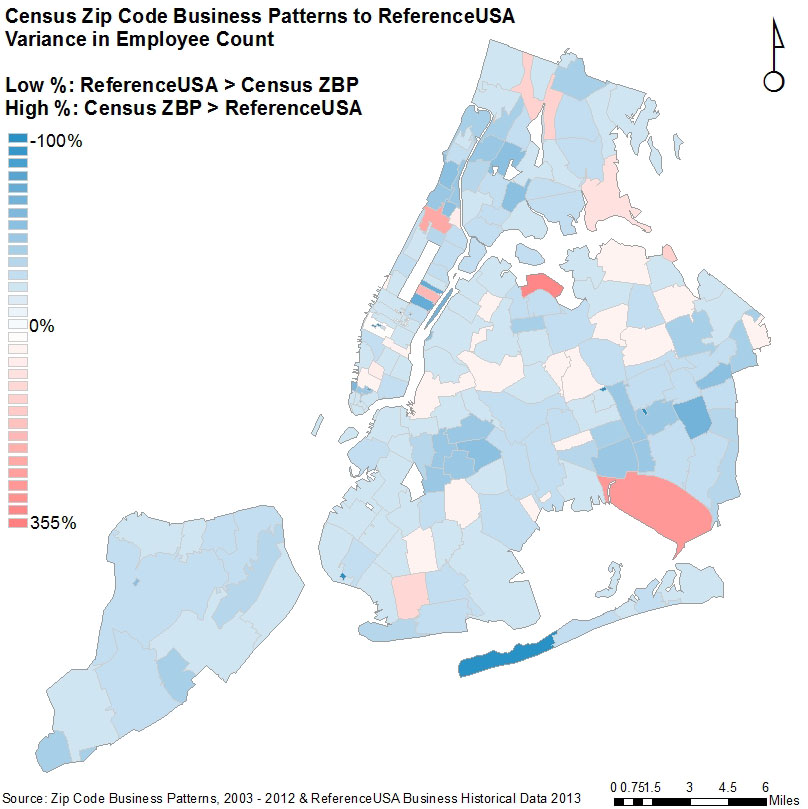
\includegraphics[width=1.0\textwidth]{7}
\pagebreak
\subsection*{Figure 8}
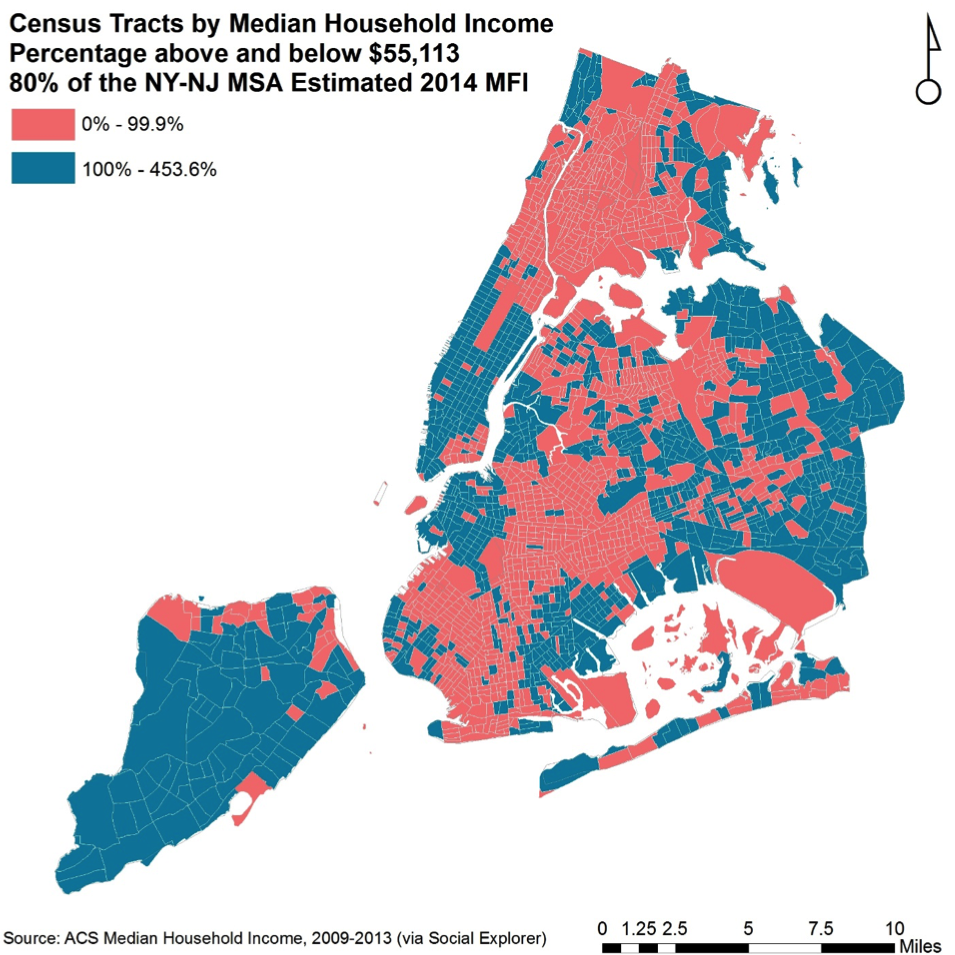
\includegraphics[width=1.0\textwidth]{8}
\pagebreak
\subsection*{Figure 9}
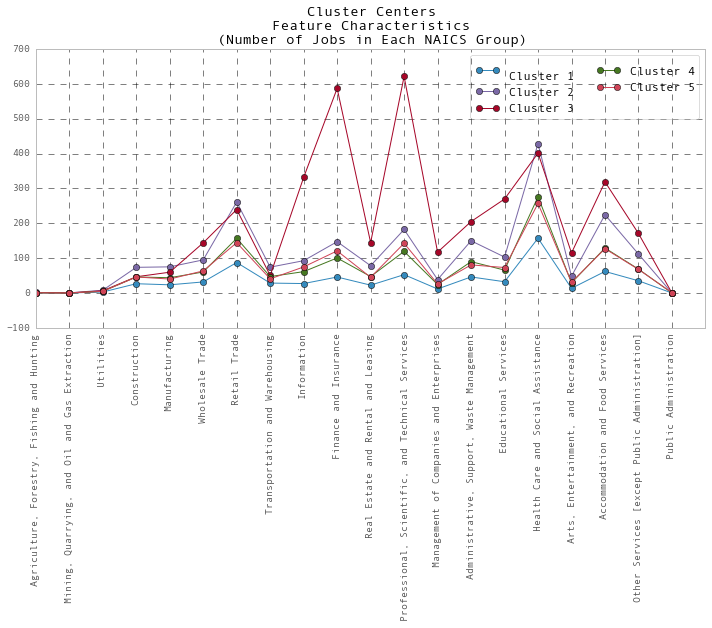
\includegraphics[width=1.0\textwidth]{9}
\subsection*{Figure 10}
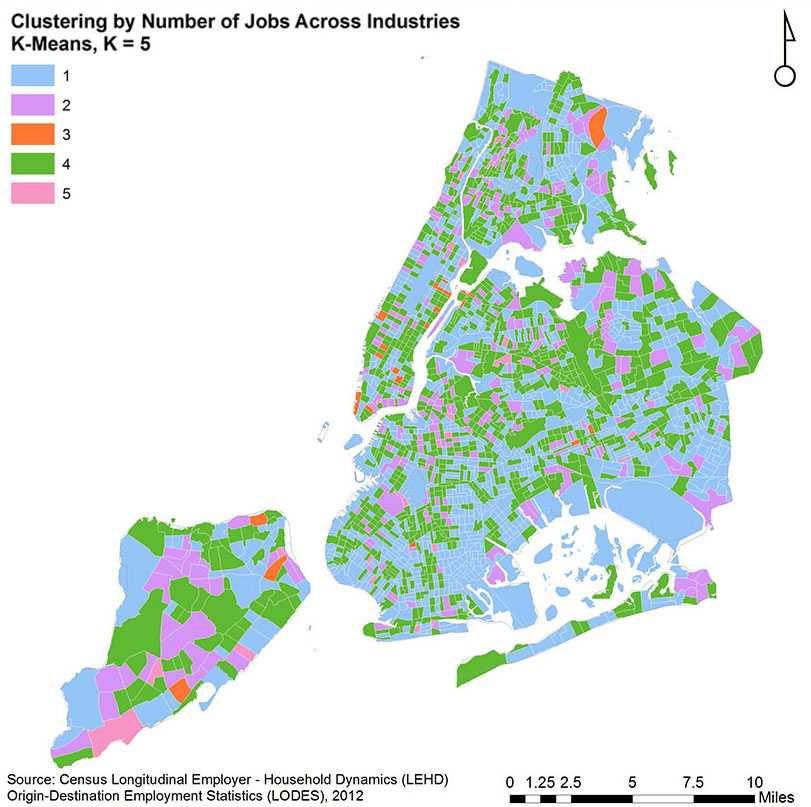
\includegraphics[width=1.0\textwidth]{10}
\subsection*{Figure 11}
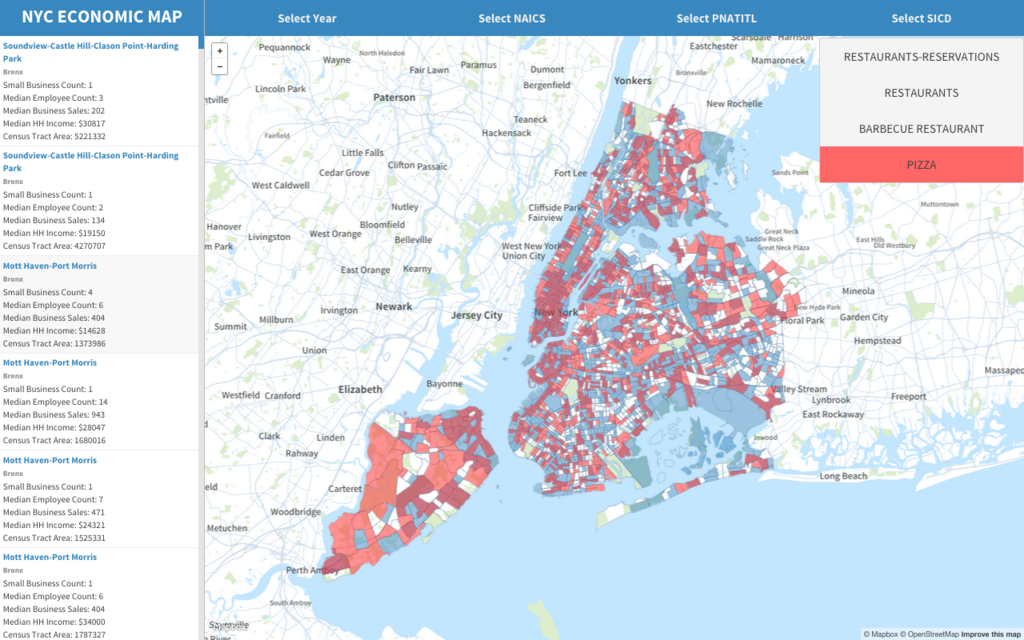
\includegraphics[width=1.0\textwidth]{11}

%----------------------------------------------------------------------------------------

\end{document}